\section{Introduction}
\label{sec:introduction}

A misread alignment flag, a 1-based coordinate parsed as 0-based,
or a silent record drop in a Variant Call Format (VCF) file
propagates from the parser to every downstream tool that consumes
its output. Independent variant-calling pipelines disagree substantially on
the same input data~\citep{orawe2013concordance}, and the
discrepancy has motivated sustained investment in pipeline-level
benchmark infrastructure such as Genome in a
Bottle~\citep{zook2019giab} and the GA4GH best-practice
protocol~\citep{krusche2019benchmarking}. These efforts grade the
joint behaviour of caller and parser under the assumption that
parsers are sound. Whether they are is rarely
tested directly. Concrete consequences are easy to find in
upstream issue trackers: htsjdk SAM regressions that accepted
reference names with delimiters disallowed by SAM 1.6 and that
over-strictly rejected reads with template lengths above
$2^{29}$, and a vcfpy regression that silently accepted symbolic
ALT alleles VCF restricts to gVCF mode. Such regressions
corrupt records that downstream callers treat as authoritative,
and the error propagates to every downstream analysis
(Figure~\ref{fig:motivation}A). The
textual specifications fix the on-disk grammar but leave many
record-level semantics to de facto consensus, so testers operate
without an external oracle~\citep{barr2015oracle}.

% Motivation figure for the BioTest paper.
% Single-column placement; full argument lives in the intro prose,
% so the caption only labels the panels.

\begin{figure}[!t]
\centering
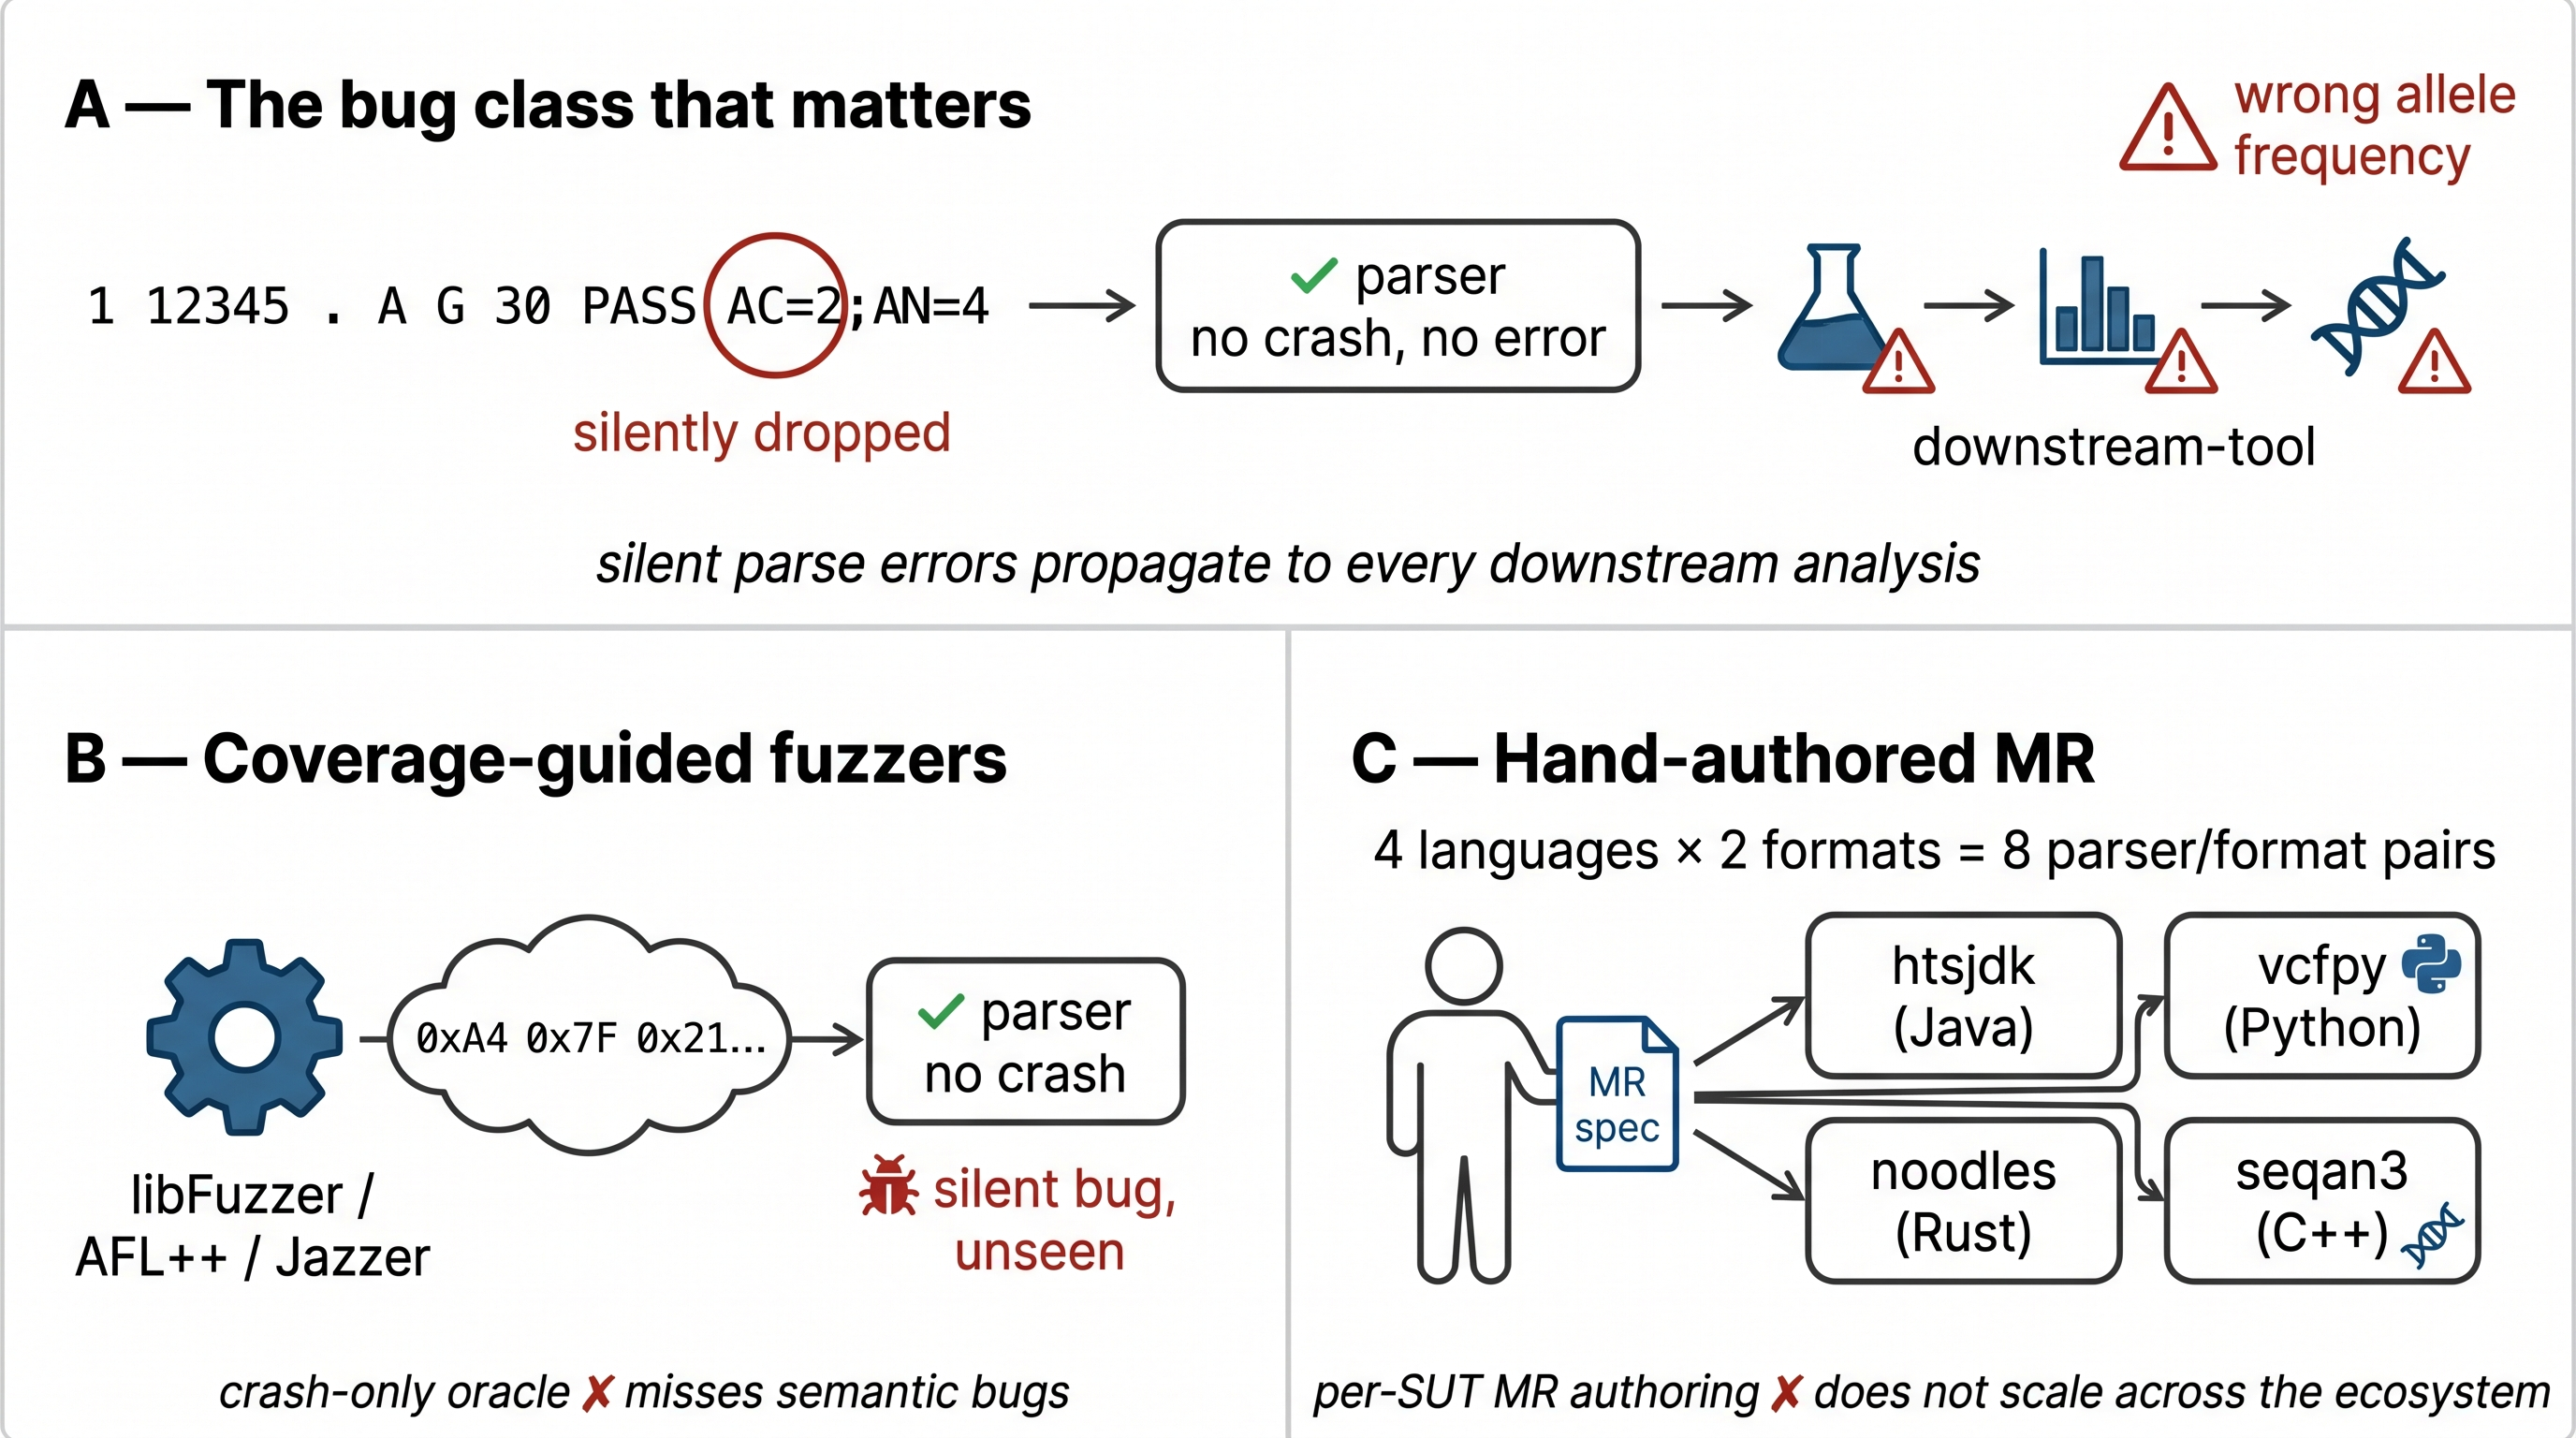
\includegraphics[width=\columnwidth]{figures/motivation.png}
\caption{The motivating gap.
\textbf{(A)}~Silent parse errors propagate to every downstream
analysis.
\textbf{(B)}~Coverage-guided fuzzers miss them under a crash-only
oracle --- these tools only flag program crashes, so the
silent-corruption bugs shown in panel~(A) go undetected.
\textbf{(C)}~Per-SUT hand-authored MRs do not scale across the
ecosystem's eight parser/format pairs.}
\label{fig:motivation}
\end{figure}


Metamorphic testing replaces ``what should the output be?'' with
relations on related
outputs~\citep{chen1998metamorphic,chen2018metamorphic}.
File-format parsers fit cleanly: identity-preserving transforms
over the spec-defined grammar yield equivalence relations
derivable from the specification rather than from the parser
source. The dominant cost is the relations themselves. The
field's open-challenge survey~\citep{chen2018metamorphic}
catalogues MR identification as the central problem, and existing
studies report relations specified per SUT by human experts in
the SUT's host language~\citep{segura2016survey}. The
bioinformatics ecosystem maintains parsers for VCF and SAM in
four host languages simultaneously (htsjdk in Java, biopython and
vcfpy in Python, noodles in Rust, seqan3 in C++), so a
hand-authored per-SUT pipeline does not scale across the eight
parser/format pairs (Figure~\ref{fig:motivation}C). The strongest
competing approaches do not scale either: coverage-guided fuzzers
require bytecode rewriting, sanitizer-instrumented builds, or
fork-server harnessing on top of the parse-and-emit shim every
fuzz tool needs, and their crash-only oracle is blind to the
silent-corruption class
that motivates this work (Figure~\ref{fig:motivation}B).

We describe \biotest{}, a metamorphic testing pipeline that
replaces the human MR-identification step with an LLM-driven,
spec-grounded mining stage. The published specification is
indexed for retrieval-augmented prompting~\citep{lewis2020rag}.
An LLM proposes identity-preserving transforms grounded in the
spec rule each transform claims to preserve, validated against a
seed corpus before admission.
Inputs flow through a corpus stack with a semantics-preserving
metamorphic tier and a per-iteration augmentation tier, and the
oracle is multi-runner consensus across $N{\geq}3$ independent
parsers. The
user's per-SUT effort is a parse-and-emit shim that emits a
canonical-JSON record set. \biotest{} adds no per-SUT MR, oracle
predicate, seed-corpus curation, or instrumentation on top.
Figure~\ref{fig:architecture} gives the visual overview.

We evaluate \biotest{} on six $(\mathrm{SUT, format})$
configurations against five coverage-guided fuzzers and a
Pure-Random floor across three axes: end-of-run line
coverage, mutation adequacy, and a real-bug
benchmark~\citep{hazimeh2020magma} of $32$ verified parser bugs
(a tool detects a bug iff some input it produces triggers the
buggy version but not the patched version). On the text-rich parsers \biotest{} leads every
coverage-guided fuzzer on line coverage and comes within
$4.2$\,pp of the strongest on mutation adequacy; it trails only
on byte-content-lenient parsers, consistent with the empirical
pattern of Klees et al.~\cite{klees2018fuzz} and
B\"ohme et al.~\cite{boehme2020boosting}. On the bug benchmark it detects $10$ of $32$ parser bugs across
three host languages (Java/htsjdk, Python/vcfpy, Rust/noodles),
where every crash-only input fuzzer in the slate detects zero.
Detection is end-to-end audited under a pre-fix\,/\,post-fix
differential predicate in the ground-truth fuzzing style of
Magma~\cite{hazimeh2020magma}, on inputs the tool's adapter
produced during the per-cell budget rather than on the
manifest's canonical proof-of-vulnerability files alone.

\textbf{Contributions.}
We contribute (i) \biotest{}, a metamorphic testing pipeline for
textual VCF and SAM parsers in which an LLM mines spec-grounded
MRs under RAG retrieval and seed-corpus validation, with parser
behaviour graded by a multi-runner consensus oracle;
(ii) a two-tier corpus stack that combines grammar-driven
metamorphic transforms with structural and lenient-byte
augmentation, plus empirical characterisation of when the
augmentation tier fails to close the gap; and (iii) a three-axis
evaluation (line coverage, mutation adequacy, $32$-bug real-bug
benchmark) under matched protocols that maps where grammar-driven
generation matches, leads, and trails coverage-guided fuzzing
under the bounded per-SUT effort envelope (\S\ref{sec:evaluation}).
